%!TeX encoding = UTF-8
%!TeX program = xelatex
\documentclass[notheorems, aspectratio=54]{beamer}
% aspectratio: 1610, 149, 54, 43(default), 32

\usepackage{latexsym}
\usepackage{amsmath,amssymb}
\usepackage{mathtools}
\usepackage{color,xcolor}
\usepackage{booktabs}
\usepackage{graphicx}
\usepackage{algorithm}
\usepackage{amsthm}
\usepackage{lmodern} % 解决 font warning
% \usepackage[UTF8]{ctex}
\usepackage{animate} % insert gif
\usepackage{hyperref}%url
\usepackage{lipsum} % To generate test text 
\usepackage{ulem} % 下划线，波浪线

\usepackage{listings} % display code on slides; don't forget [fragile] option after \begin{frame}

% ----------------------------------------------
% tikx
\usepackage{framed}
\usepackage{tikz}
\usepackage{pgf}
\usetikzlibrary{calc,trees,positioning,arrows,chains,shapes.geometric,%
    decorations.pathreplacing,decorations.pathmorphing,shapes,%
    matrix,shapes.symbols}
\pgfmathsetseed{1} % To have predictable results
% Define a background layer, in which the parchment shape is drawn
\pgfdeclarelayer{background}
\pgfsetlayers{background,main}

% define styles for the normal border and the torn border
\tikzset{
  normal border/.style={orange!30!black!10, decorate, 
     decoration={random steps, segment length=2.5cm, amplitude=.7mm}},
  torn border/.style={orange!30!black!5, decorate, 
     decoration={random steps, segment length=.5cm, amplitude=1.7mm}}}

% Macro to draw the shape behind the text, when it fits completly in the
% page
\def\parchmentframe#1{
\tikz{
  \node[inner sep=2em] (A) {#1};  % Draw the text of the node
  \begin{pgfonlayer}{background}  % Draw the shape behind
  \fill[normal border] 
        (A.south east) -- (A.south west) -- 
        (A.north west) -- (A.north east) -- cycle;
  \end{pgfonlayer}}}

% Macro to draw the shape, when the text will continue in next page
\def\parchmentframetop#1{
\tikz{
  \node[inner sep=2em] (A) {#1};    % Draw the text of the node
  \begin{pgfonlayer}{background}    
  \fill[normal border]              % Draw the ``complete shape'' behind
        (A.south east) -- (A.south west) -- 
        (A.north west) -- (A.north east) -- cycle;
  \fill[torn border]                % Add the torn lower border
        ($(A.south east)-(0,.2)$) -- ($(A.south west)-(0,.2)$) -- 
        ($(A.south west)+(0,.2)$) -- ($(A.south east)+(0,.2)$) -- cycle;
  \end{pgfonlayer}}}

% Macro to draw the shape, when the text continues from previous page
\def\parchmentframebottom#1{
\tikz{
  \node[inner sep=2em] (A) {#1};   % Draw the text of the node
  \begin{pgfonlayer}{background}   
  \fill[normal border]             % Draw the ``complete shape'' behind
        (A.south east) -- (A.south west) -- 
        (A.north west) -- (A.north east) -- cycle;
  \fill[torn border]               % Add the torn upper border
        ($(A.north east)-(0,.2)$) -- ($(A.north west)-(0,.2)$) -- 
        ($(A.north west)+(0,.2)$) -- ($(A.north east)+(0,.2)$) -- cycle;
  \end{pgfonlayer}}}

% Macro to draw the shape, when both the text continues from previous page
% and it will continue in next page
\def\parchmentframemiddle#1{
\tikz{
  \node[inner sep=2em] (A) {#1};   % Draw the text of the node
  \begin{pgfonlayer}{background}   
  \fill[normal border]             % Draw the ``complete shape'' behind
        (A.south east) -- (A.south west) -- 
        (A.north west) -- (A.north east) -- cycle;
  \fill[torn border]               % Add the torn lower border
        ($(A.south east)-(0,.2)$) -- ($(A.south west)-(0,.2)$) -- 
        ($(A.south west)+(0,.2)$) -- ($(A.south east)+(0,.2)$) -- cycle;
  \fill[torn border]               % Add the torn upper border
        ($(A.north east)-(0,.2)$) -- ($(A.north west)-(0,.2)$) -- 
        ($(A.north west)+(0,.2)$) -- ($(A.north east)+(0,.2)$) -- cycle;
  \end{pgfonlayer}}}

% Define the environment which puts the frame
% In this case, the environment also accepts an argument with an optional
% title (which defaults to ``Example'', which is typeset in a box overlaid
% on the top border
\newenvironment{parchment}[1][Example]{%
  \def\FrameCommand{\parchmentframe}%
  \def\FirstFrameCommand{\parchmentframetop}%
  \def\LastFrameCommand{\parchmentframebottom}%
  \def\MidFrameCommand{\parchmentframemiddle}%
  \vskip\baselineskip
  \MakeFramed {\FrameRestore}
  \noindent\tikz\node[inner sep=1ex, draw=black!20,fill=white, 
          anchor=west, overlay] at (0em, 2em) {\sffamily#1};\par}%
{\endMakeFramed}

% ----------------------------------------------

\mode<presentation>{
    \usetheme{CambridgeUS}
    % Boadilla CambridgeUS
    % default Antibes Berlin Copenhagen
    % Madrid Montpelier Ilmenau Malmoe
    % Berkeley Singapore Warsaw
    \usecolortheme{beaver}
    % beetle, beaver, orchid, whale, dolphin
    \useoutertheme{infolines}
    % infolines miniframes shadow sidebar smoothbars smoothtree split tree
    \useinnertheme{circles}
    % circles, rectanges, rounded, inmargin
}
% 设置 block 颜色
\setbeamercolor{block title}{bg=red!30,fg=white}

\newcommand{\reditem}[1]{\setbeamercolor{item}{fg=red}\item #1}

% 缩放公式大小
\newcommand*{\Scale}[2][4]{\scalebox{#1}{\ensuremath{#2}}}

% 解决 font warning
\renewcommand\textbullet{\ensuremath{\bullet}}

% ---------------------------------------------------------------------
% flow chart
\tikzset{
    >=stealth',
    punktchain/.style={
        rectangle, 
        rounded corners, 
        % fill=black!10,
        draw=white, very thick,
        text width=6em,
        minimum height=2em, 
        text centered, 
        on chain
    },
    largepunktchain/.style={
        rectangle,
        rounded corners,
        draw=white, very thick,
        text width=10em,
        minimum height=2em,
        on chain
    },
    line/.style={draw, thick, <-},
    element/.style={
        tape,
        top color=white,
        bottom color=blue!50!black!60!,
        minimum width=6em,
        draw=blue!40!black!90, very thick,
        text width=6em, 
        minimum height=2em, 
        text centered, 
        on chain
    },
    every join/.style={->, thick,shorten >=1pt},
    decoration={brace},
    tuborg/.style={decorate},
    tubnode/.style={midway, right=2pt},
    font={\fontsize{10pt}{12}\selectfont},
}
% ---------------------------------------------------------------------

% code setting
\lstset{
    language=C++,
    basicstyle=\ttfamily\footnotesize,
    keywordstyle=\color{red},
    breaklines=true,
    xleftmargin=2em,
    numbers=left,
    numberstyle=\color[RGB]{222,155,81},
    frame=leftline,
    tabsize=4,
    breakatwhitespace=false,
    showspaces=false,               
    showstringspaces=false,
    showtabs=false,
    morekeywords={Str, Num, List},
}

% ---------------------------------------------------------------------

%% preamble
\title[An image is worth $16 \times 16$ words]{An image is worth $16 \times 16$ words: \\
Transformers for Image Recognition at Scale~\cite{image2021}}
% \subtitle{The subtitle}
\author{Jincheng Xu}
\institute[SCU]{2023141460134}

% -------------------------------------------------------------

\begin{document}

%% title frame
%% title frame
\begin{frame}
    \titlepage
    \vspace{1.2em}
    {\scriptsize \hspace{1.5em}ViT is the first work to prove that a pure Transformer can achieve state-of-the-art performance in image classification. ViT treats each image as a sequence of tokens and then feeds them to multiple Transformer layers to make the classification.~\cite{seg2021}\par}
\end{frame}

\begin{frame}
    \begin{columns}[T]
        \column{0.5\textwidth}
            \begin{figure}[htbp]
                \centering
                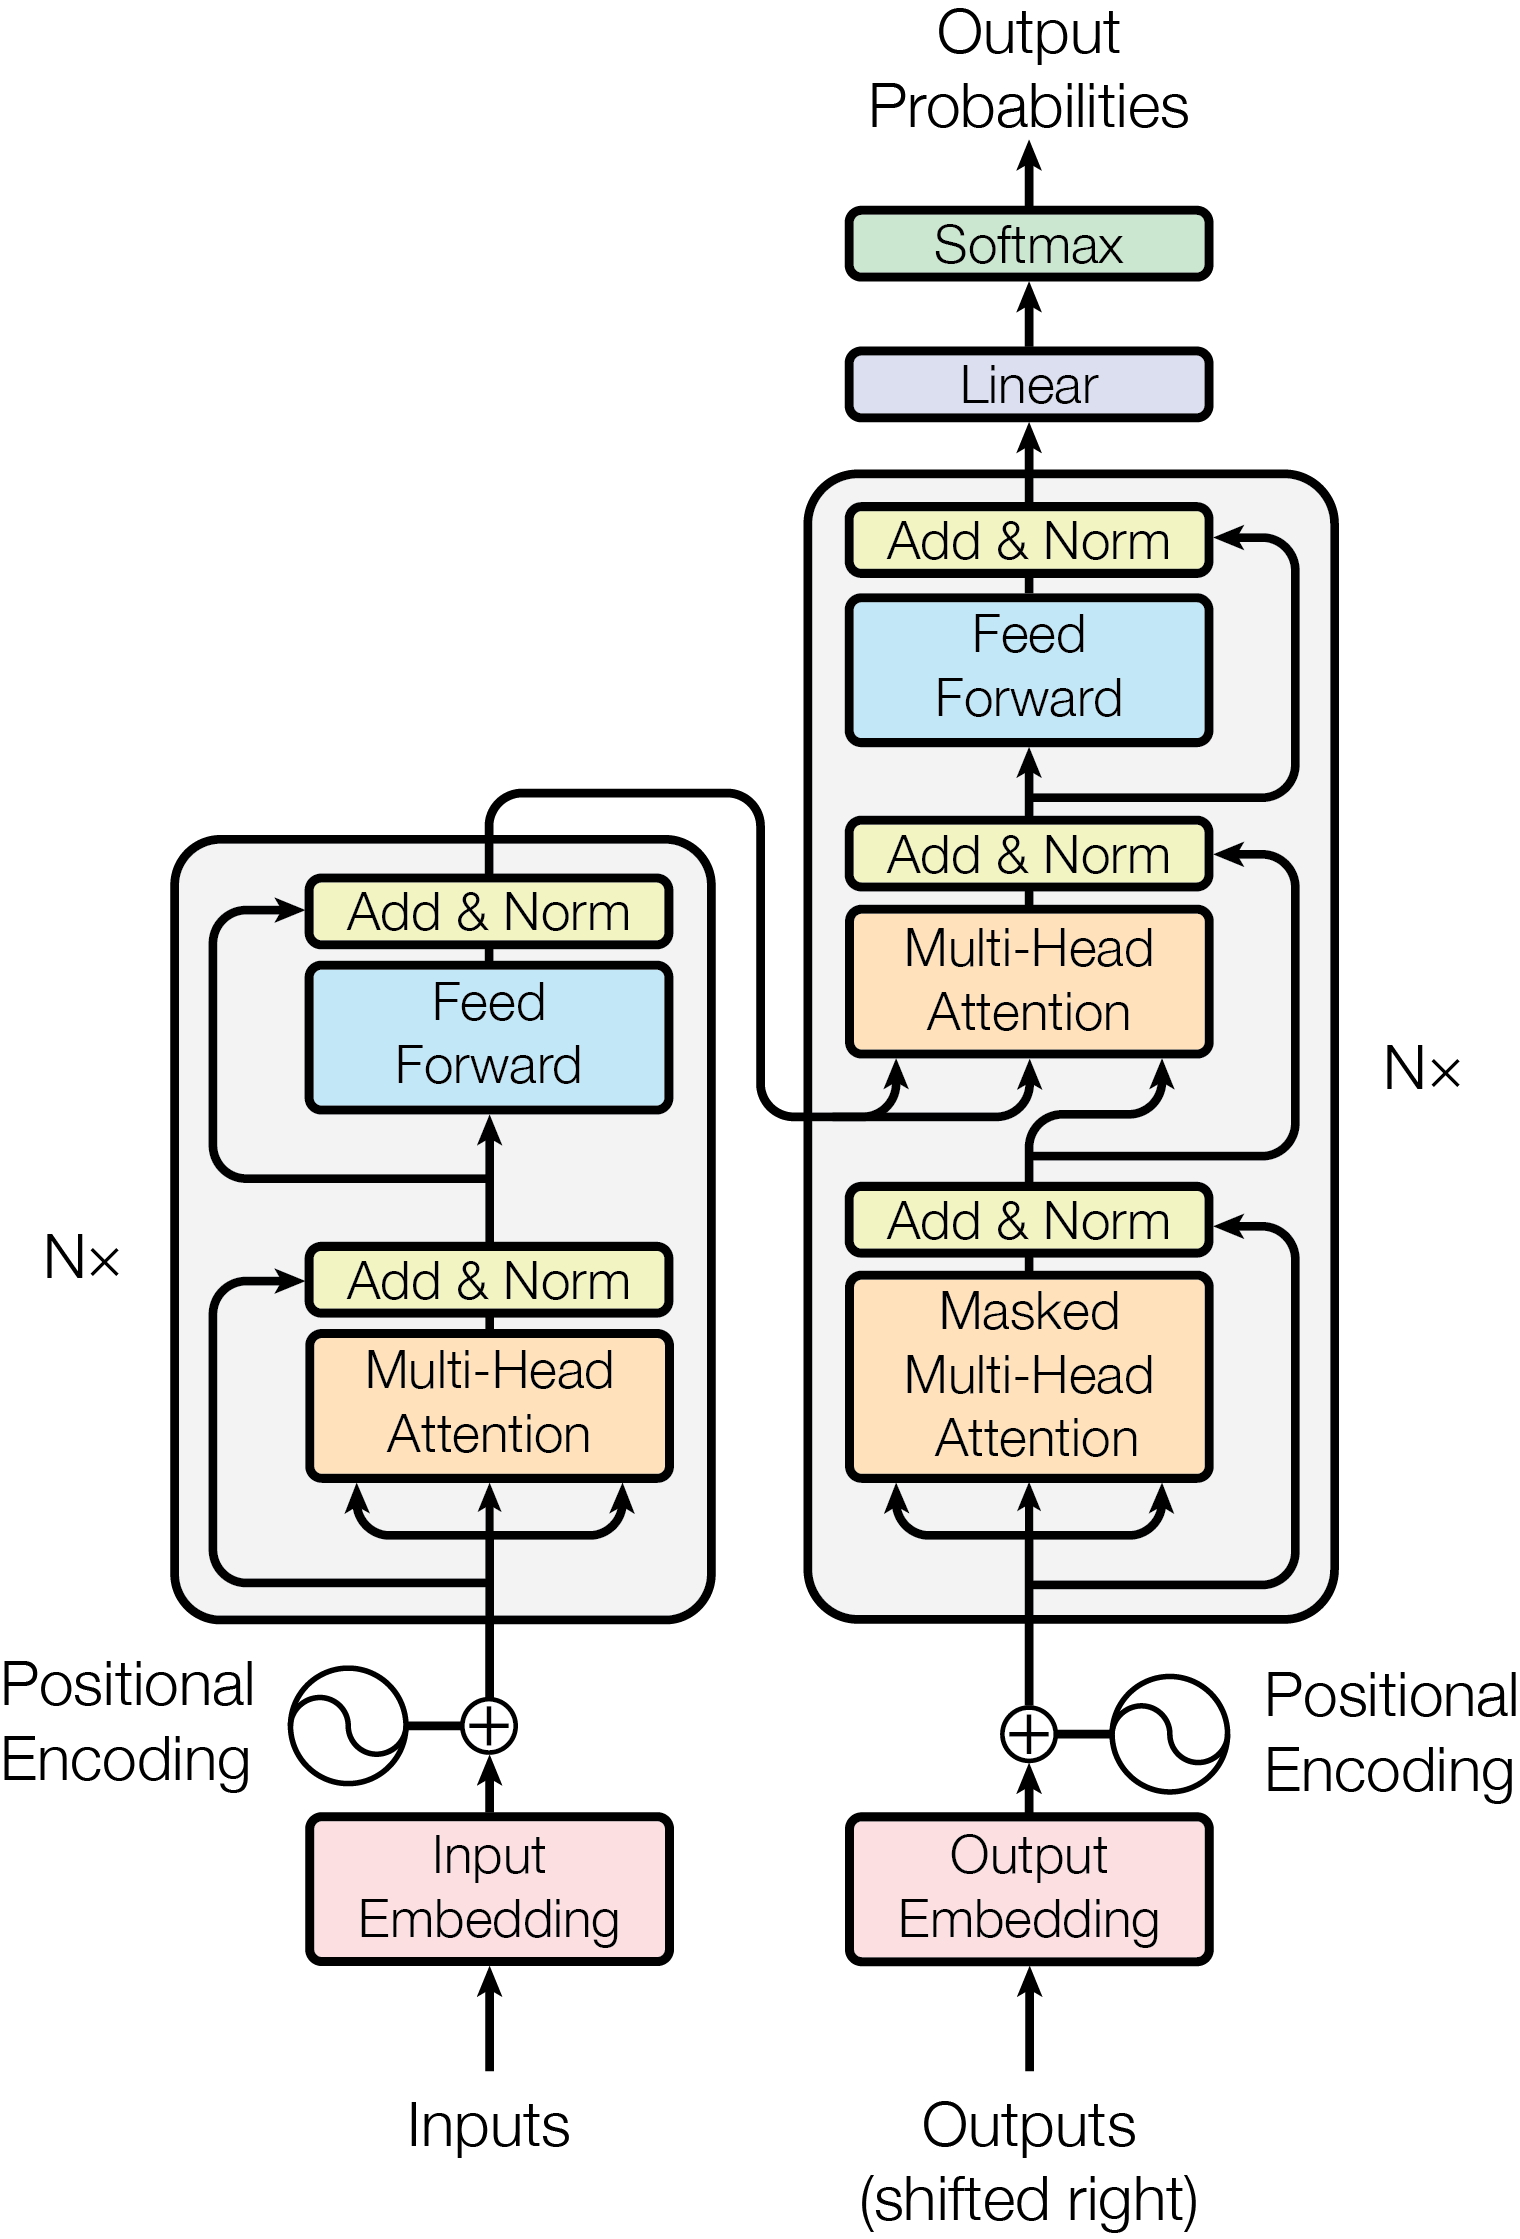
\includegraphics[width=0.65\textwidth]{fig/trans.png}
                \caption{Transformer}
                \label{trans}
            \end{figure}

        \column{0.5\textwidth}
        % 右边放文字（可选）
        \textbf{Prediction in Conclusion}\\
        \hspace{1.5em}We are excited about the future of attention-based models and plan to apply them to other tasks. We plan to extend the Transformer to problems involving input and output modalities other than text and to investigate local, restricted attention mechanisms to efficiently handle large inputs and outputs such as images, audio and video.~\cite{attn2017}
    \end{columns}
\end{frame}

\begin{frame}{Motivation}
    \begin{itemize}
        \item \textbf{Superiority of Transformer-based Model}\\
        \begin{itemize}
            \item No sign of saturating performance
            \item Computational efficiency
            \item Scalability
        \end{itemize}
    \end{itemize}
    \begin{itemize}
        \item \textbf{Computer Vision}\\
        Convolutional architectures remain dominant
    \end{itemize}
   \begin{figure}[htbp]
        \centering
        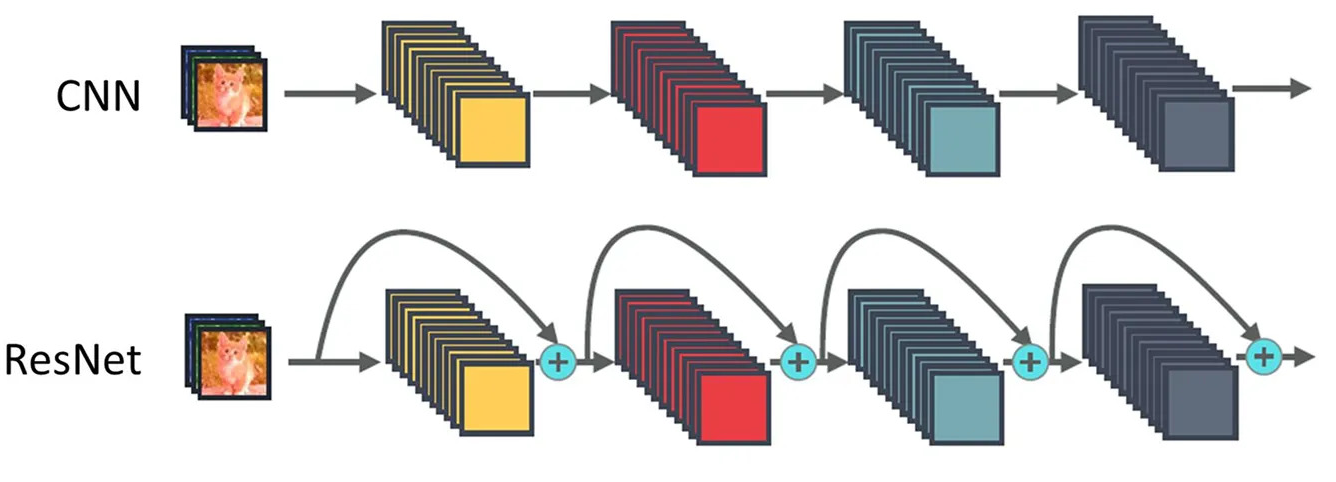
\includegraphics[width=0.8\textwidth]{fig/ResNet.png}
        \caption{CNNs and ResNet}
        \label{CNN}
    \end{figure}
\end{frame}



\begin{frame}{Related Work}
    \begin{enumerate}
        \item Combining CNN-like architectures with self-attention~\cite{hybrid2020}
        \item Replacing the convolutions entirely with Transformers~\cite{entire2020}\\
        {\hspace{1.5em}\small Theoretically efficient,have not yet been scaled effectively on modern hardware accelerators}
    \end{enumerate}
    
    \begin{figure}[htbp]
        \centering
        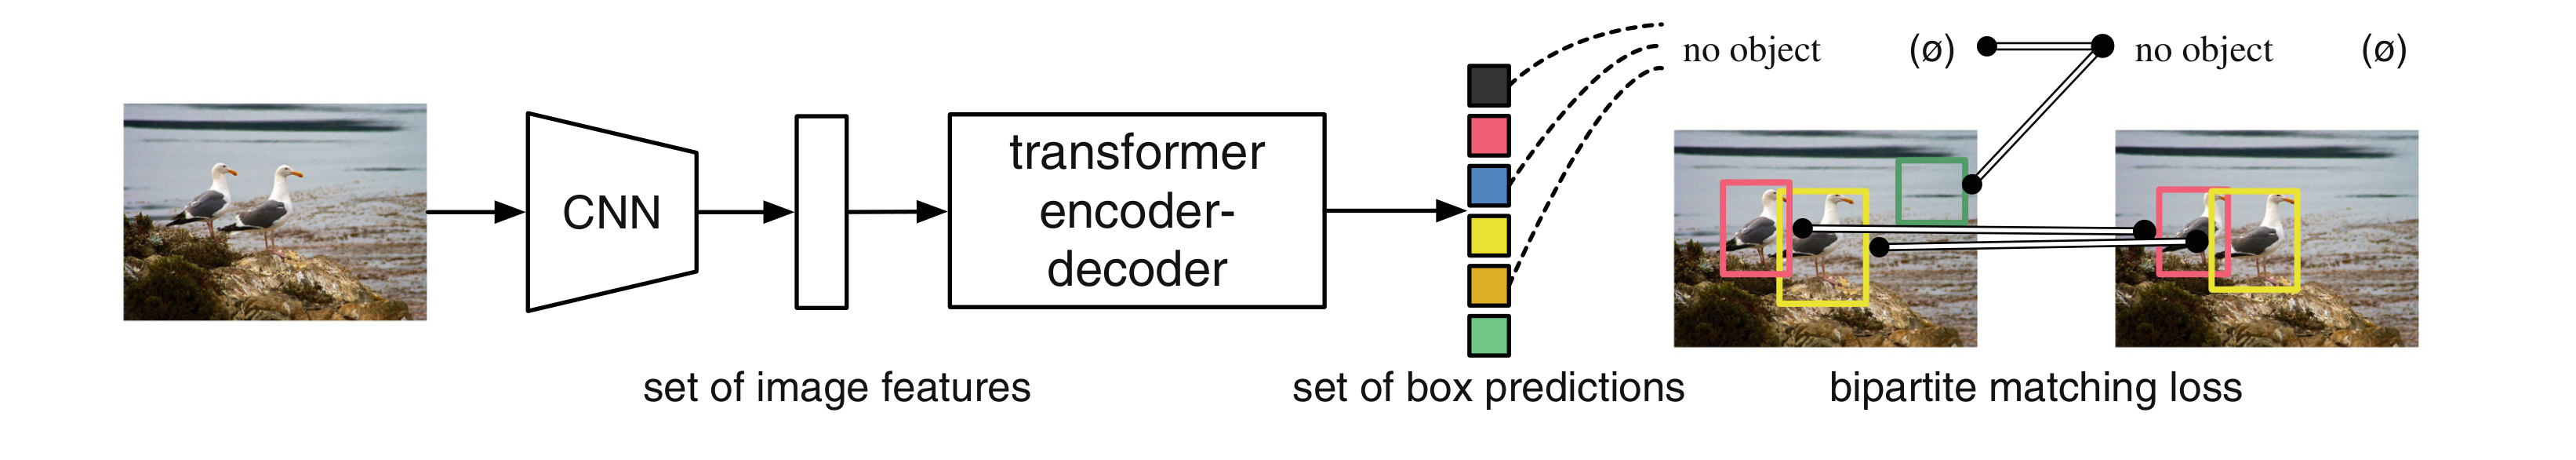
\includegraphics[width=0.6\textwidth]{fig/hybrid.jpg}
        \caption{Hybrid structure}
        \label{hybrid}
    \end{figure}
    \vspace{-1em}
    \begin{figure}[htbp]
        \centering
        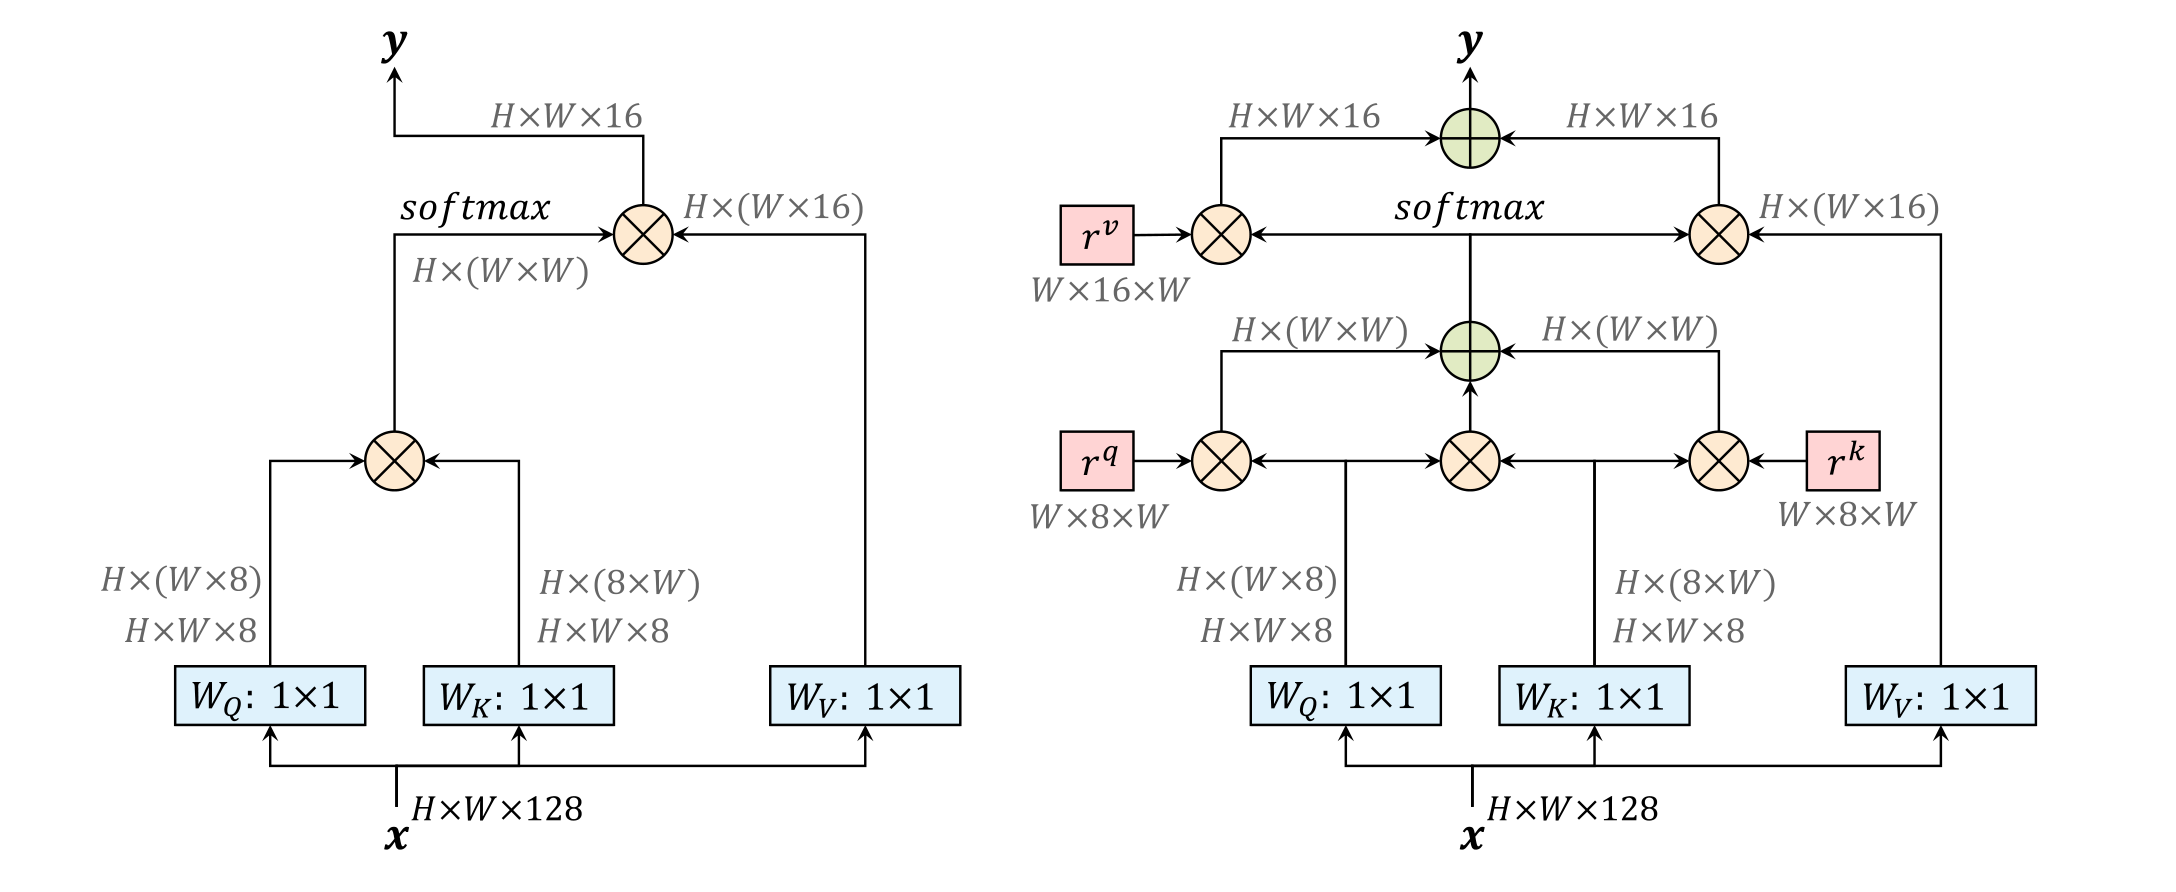
\includegraphics[width=0.6\textwidth]{fig/entire.png}
        \vspace{-1em}
        \caption{Entirely replace}
        \label{entire}
    \end{figure}

\end{frame}

\begin{frame}{Superiority of ViT}
    \begin{enumerate}
        \item Pure transformer on image classification tasks with the fewest possible modifications
        \item Large scale training trumps inductive bias:\\\hspace{1.5em}ViT approaches or beats state of the art on multiple image recognition benchmarks.
        \item Large attention distance across image
    \end{enumerate}
    
    \begin{figure}[htbp]
        \centering
        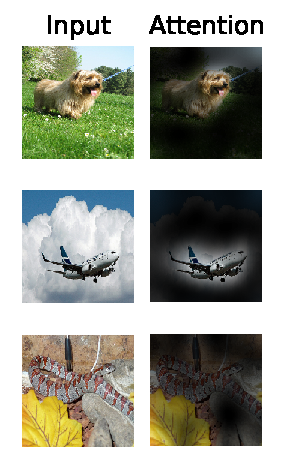
\includegraphics[width=0.2\textwidth]{fig/attn_dis.pdf}
        \vspace{-0.8em}
        \caption{As depth increases, attention distance increases for all heads. In the second half of the network, most heads attend widely across tokens.}
        \label{attn_dis.pdf}
    \end{figure}
\end{frame}

\begin{frame}
    \begin{table}[htpb]
        \centering
        \tiny
        \caption{\scriptsize Model Performance Across Datasets and Training Efficiency}\label{tab:model_perf}
        \vspace{-1em}
        \begin{tabular}{l *{5}{c}}
            \toprule
            Dataset & Ours-JFT (ViT-H/14) & Ours-JFT (ViT-L/16) & Ours-I21k (ViT-L/16) & BiT-L (ResNet152x4) & Noisy Student (EfficientNet-L2) \\
            \midrule
            ImageNet & 88.55±0.04& 87.76±0.03& 85.30±0.02& 87.54±0.02& 88.4/88.5
            
            \\
            ImageNet ReaL & 90.72±0.05& 90.54±0.03& 88.62±0.05& 90.54& 90.55\\
            CIFAR-10 & 99.50±0.06& 99.42±0.03& 99.15±0.03& 99.37±0.06& — \\
            CIFAR-100 & 94.55±0.04& 93.90±0.05& 93.25±0.05& 93.51±0.08& — \\
            Oxford-IIIT Pets & 97.56±0.03& 97.32±0.11& 94.67±0.15& 96.62±0.23& — \\
            Oxford Flowers-102 & 99.68±0.02& 99.74±0.00& 99.61±0.02& 99.63±0.03& — \\
            VTAB (19 tasks) & 77.63±0.23& 76.28±0.46& 72.72±0.21& 76.29±1.70& — \\
            TPUv3-core-days & 2.5k & 0.68k & 0.23k & 9.9k & 12.3k \\
            \bottomrule
        \end{tabular}
    \end{table}

    \begin{figure}[htbp]
        \centering
        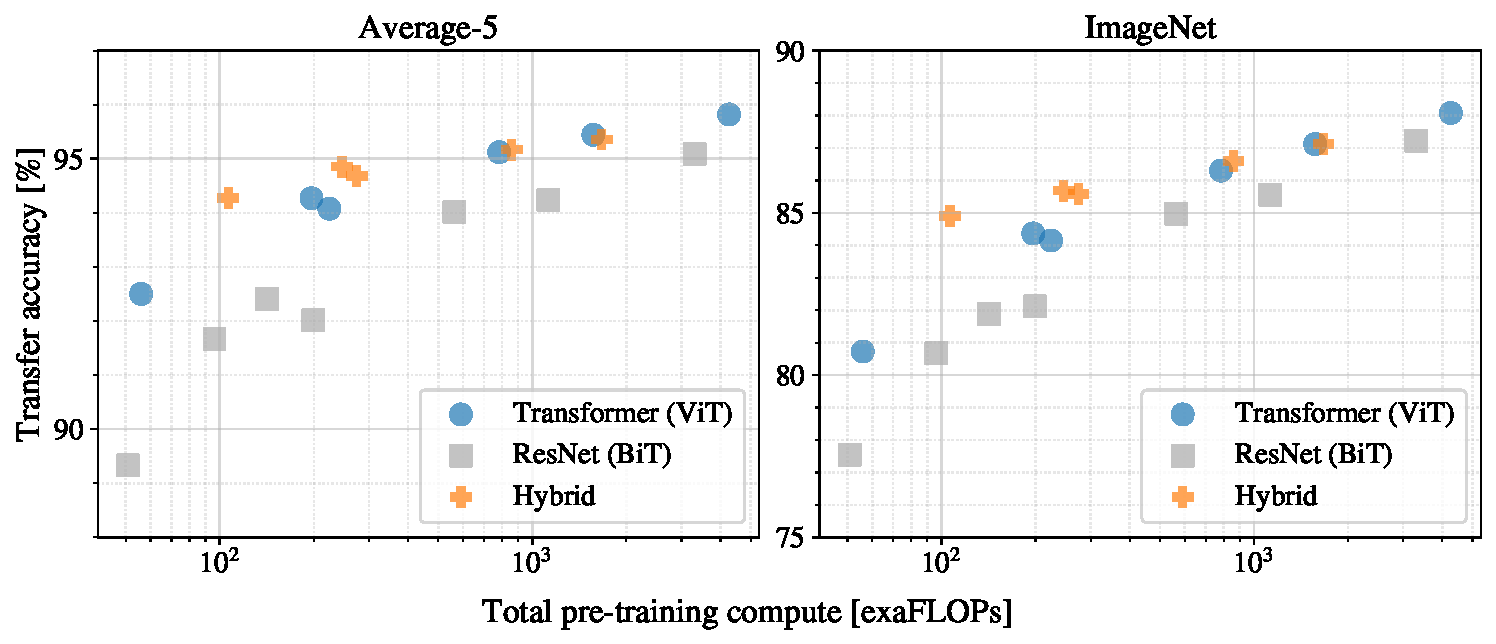
\includegraphics[width=0.8\textwidth]{fig/versus.pdf}
        \vspace{-1em}
        \caption{Performance versus pre-training compute for different architectures: Vision Transformers, ResNets, and hybrids.}
        \label{versus}
    \end{figure}

\end{frame}

\begin{frame}{Structure} 
    \begin{figure}
        \centering
        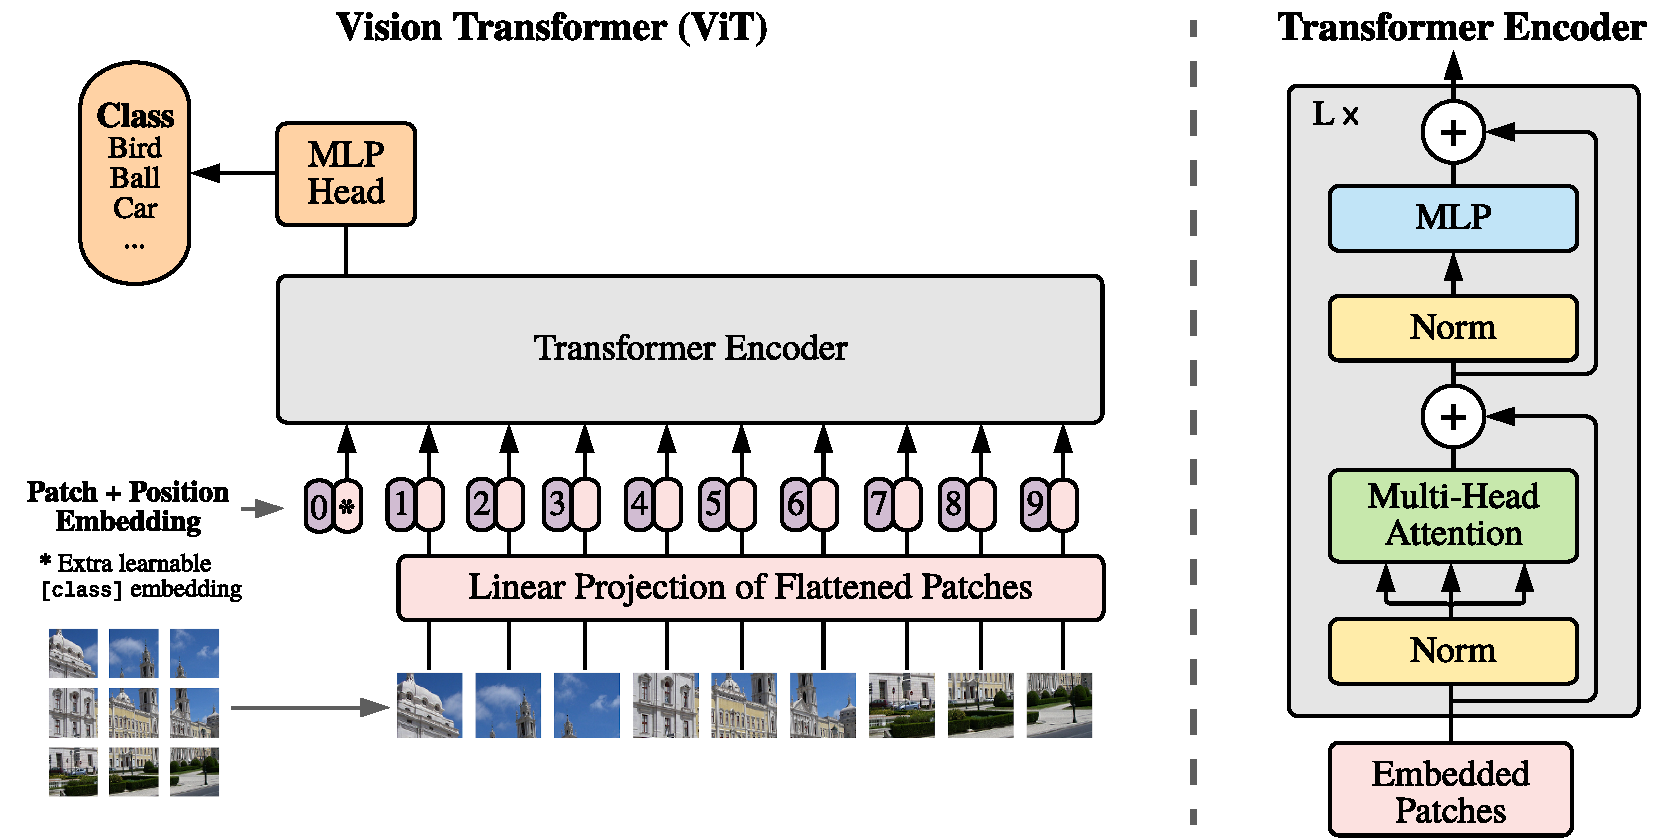
\includegraphics[width=1\textwidth]{fig/1.pdf}
        \caption{Model overview}
    \end{figure}
\end{frame}


\begin{frame}{Method}
    \begin{columns}[T]
        \column{0.33\textwidth}
        \begin{figure}
            \raggedright
            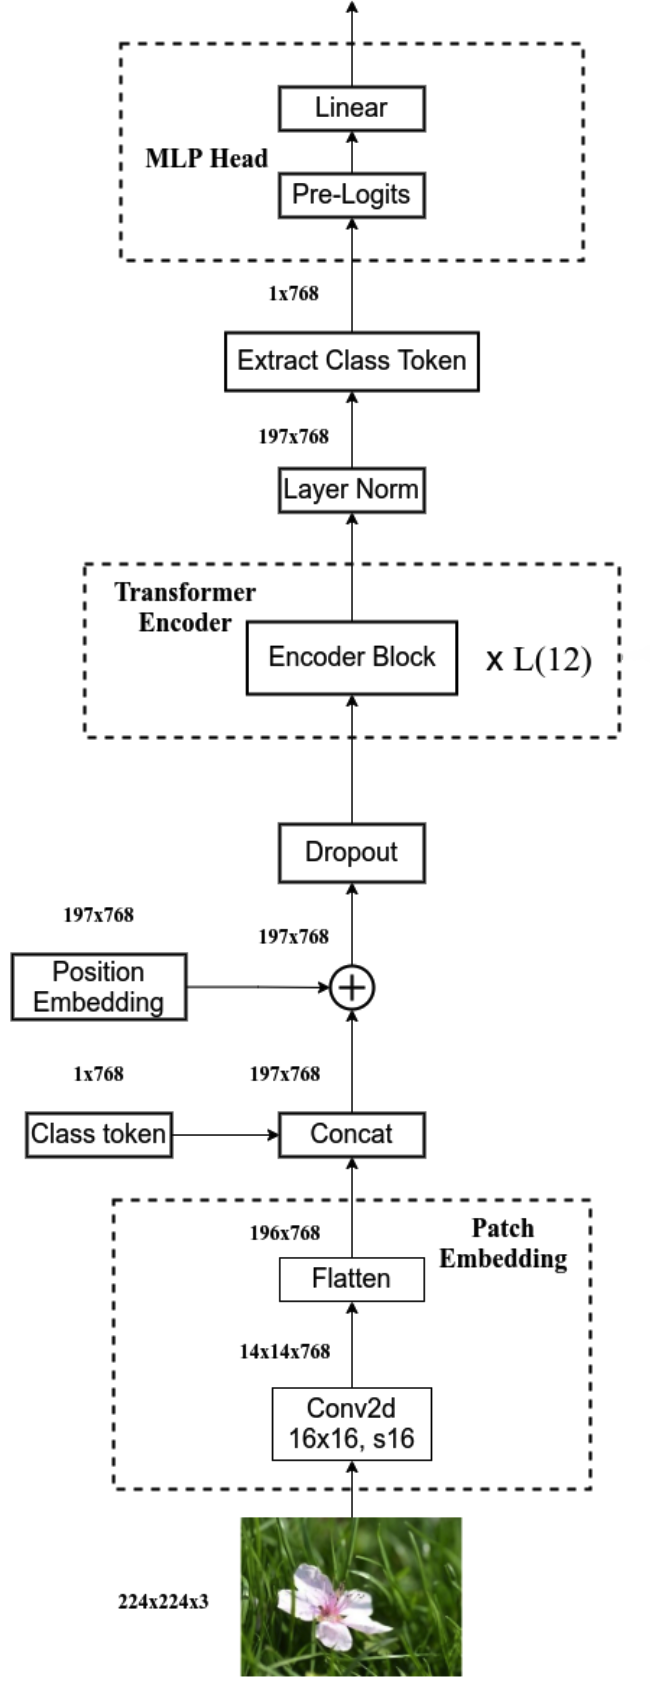
\includegraphics[width=0.7\linewidth]{fig/2.png}
        \end{figure}

        \column{0.67\textwidth}
        % 右边放文字（可选）
        \textbf{Data Preprocessing}
        \begin{enumerate}
            \item Split an image into fixed-size patches
            \item Flatten the patches
            \item Linearly embed each of them with a trainable linear projection
            \item Adding an extra learnable “classification token” to the sequence
            \item Add position embeddings
            {
            \[     \mathbf{z}_0=\left[\mathbf{x}_{\text{class}};\mathbf{x}_p^1\mathbf{E};\cdots;\mathbf{x}_p^N\mathbf{E}\right]+\mathbf{E}_{\text{pos}}
            \]

            \[
            \mathbf{E}\in\mathbb{R}^{(P^2\cdot C)\times D},
            \mathbf{E}_{\text{pos}}\in\mathbb{R}^{(N+1)\times D}
            \]
            }
            
        \end{enumerate}
    \end{columns}
\end{frame}

\begin{frame}{Method}
\textbf{Inductive bias}
    \begin{itemize}
        \item In ViT, the two-dimensional neighborhood structure is used very sparingly:
        \begin{itemize}
            \item In the beginning of the model by cutting the image into patches and at fine-tuning time for adjusting the position embeddings for images of different resolution.
        \end{itemize}
    \end{itemize}
{\scriptsize
\begin{table}
\centering
\begin{tabular}{lccc} 
    \toprule % 顶部粗线
    Pos. Emb. & Default/Stem & Every Layer & Every Layer-Shared \\
    \midrule % 中间细线
    No Pos. Emb. & 0.61382 & \text{N/A} & \text{N/A} \\
    1-D Pos. Emb. & 0.64206 & 0.63964 & 0.64292 \\
    2-D Pos. Emb. & 0.64001 & 0.64046 & 0.64022 \\
    Rel. Pos. Emb. & 0.64032 & \text{N/A} & \text{N/A} \\
    \bottomrule % 底部粗线
\end{tabular}
    
\end{table}
}
\end{frame}


\begin{frame}{Limitation}
    \begin{itemize}
        \item Performance decreases when processing different resolution image\\
        {\small 
        \hspace{1.5em} The Vision Transformer can handle arbitrary sequence lengths (up to memory constraints), however, the pre-trained position embeddings may no longer be meaningful.~\cite{image2021}
        SegFormer comprises a novel hierarchically structured Transformer encoder which outputs multiscale features. It does not need positional encoding, thereby avoiding the interpolation of positional codes which leads to decreased performance when the testing resolution differs from training.~\cite{seg2021}\\
        }
        
    \end{itemize}
    \begin{figure}
        \centering
        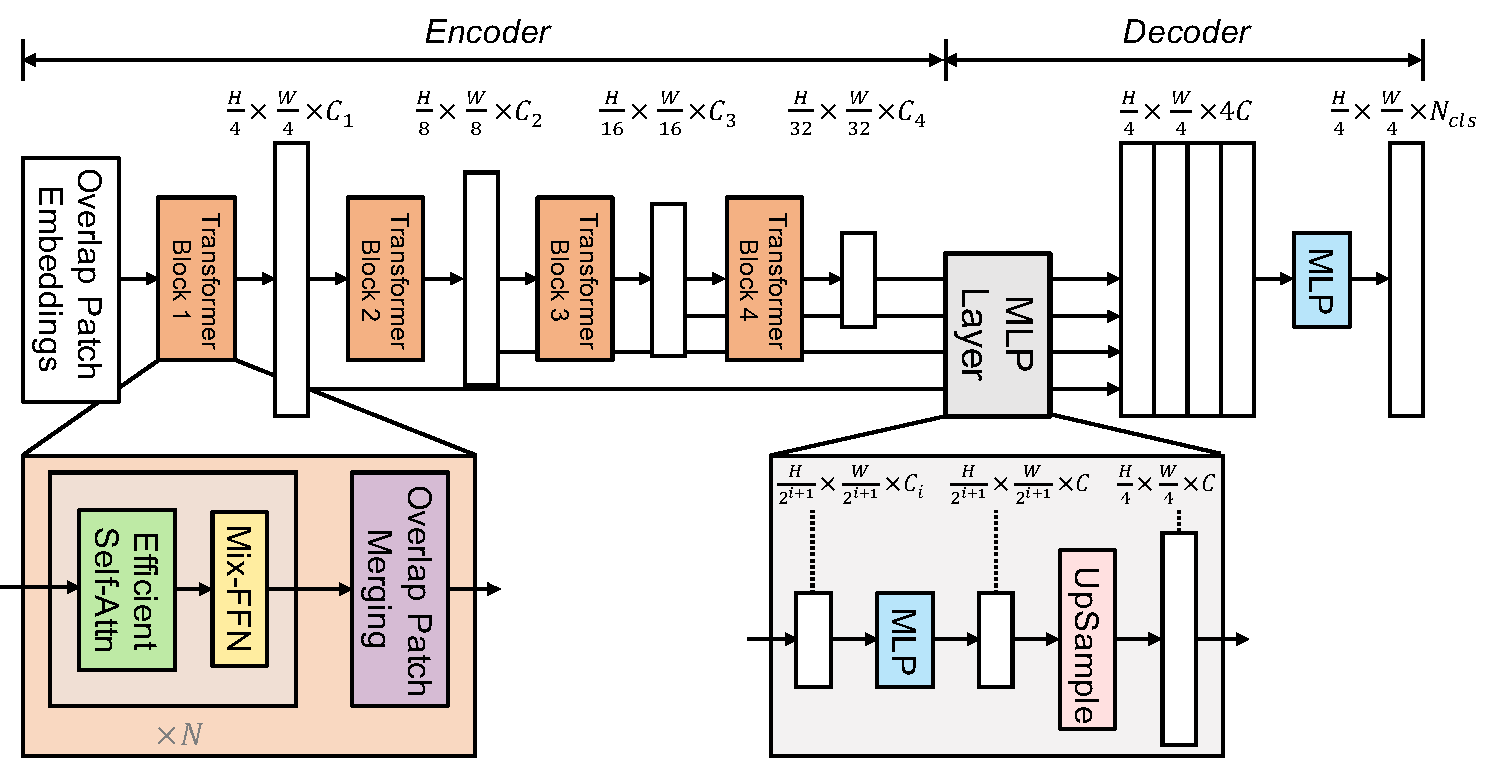
\includegraphics[width=0.65\textwidth]{fig/segformer.pdf}
        \vspace{-1em}
        \caption{SegFormer}
    \end{figure}
\end{frame}

\begin{frame}{Limitation}
    \begin{itemize}
        \item Reduced image-specific inductive bias\\
        {\small
        \hspace{1.5em} Vision Transformer has much less image-specific inductive bias than CNNs.In CNNs, locality, two-dimensional neighborhood structure, and translation equivariance are baked into each layer throughout the whole model.~\cite{image2021}
        }
    \end{itemize}
    \begin{figure}
        \centering
        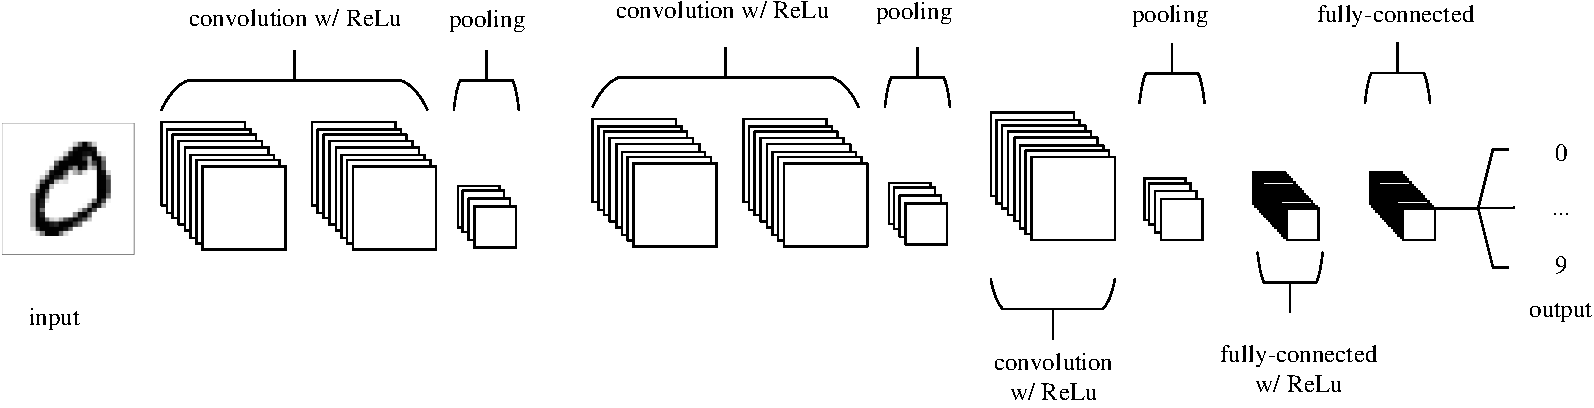
\includegraphics[width=0.8\textwidth]{fig/CNN.pdf}
        \caption{CNN}
    \end{figure}
\end{frame}
%% normal frame

\begin{frame}[allowframebreaks]{References}
    \textbf{Thanks for Listening!}
    {\tiny
    \bibliographystyle{plain}
    \bibliography{ref}
    \vspace{1em}
    \url{【ViT Lecture by LiMu】https://www.bilibili.com/video/BV15P4y137jb?vd_source=47ea6e11f644e8fae50997c63140dd52}
    }
    
\end{frame}


\end{document}